% ---------------------------------------------------------------------------
% ---------------------------------------------------------------------------
% Junção de templates encontrados no Overleaf
% facilitando a vida do aluno de pós da UFABC
% Modelo LaTex para preparação do documento final de Dissertação de Mestrado
% ninguém do programa de pós da informação validou se presta
% ---------------------------------------------------------------------------
% ---------------------------------------------------------------------------

\documentclass[
% -- opções da classe memoir --
12pt,					% tamanho da fonte
openright,				% capítulos começam em pág ímpar (insere página vazia caso preciso)
twoside,					% para impressão em verso e anverso. Oposto a oneside
a4paper,					% tamanho do papel. 
% -- opções da classe abntex2 --
%chapter=TITLE,			% títulos de capítulos convertidos em letras maiúsculas
%section=TITLE,			% títulos de seções convertidos em letras maiúsculas
%subsection=TITLE,		% títulos de subseções convertidos em letras maiúsculas
%subsubsection=TITLE,	% títulos de subsubseções convertidos em letras maiúsculas
% -- opções do pacote babel --
english,					% idioma adicional para hifenização
%french,					% idioma adicional para hifenização
%spanish,				% idioma adicional para hifenização
brazil					% o último idioma é o principal do documento
]{abntex2}

% ---------------------
% Pacotes OBRIGATÓRIOS
% ---------------------
\usepackage{lmodern}				% Usa a fonte Latin Modern			
\usepackage[T1]{fontenc}			% Selecao de codigos de fonte.
\usepackage[utf8]{inputenc}		% Codificacao do documento (conversão automática dos acentos)
\usepackage{lastpage}			% Usado pela Ficha catalográfica
\usepackage{indentfirst}			% Indenta o primeiro parágrafo de cada seção.
\usepackage{color}				% Controle das cores
\usepackage{graphicx}	% Inclusão de gráficos
\usepackage{epsfig,subfig}		% Inclusão de figuras
\usepackage{microtype} 			% Melhorias de justificação
% ---------------------

% ---------------------
% Pacotes ADICIONAIS
% ---------------------
\usepackage{lipsum}						% Geração de dummy text
\usepackage{amsmath,amssymb,mathrsfs}	% Comandos matemáticos avançados 
\usepackage{setspace}  					% Para permitir espaçamento simples, 1 1/2 e duplo
\usepackage{verbatim}					% Para poder usar o ambiente "comment"
\usepackage{tabularx} 					% Para poder ter tabelas com colunas de largura auto-ajustável
\usepackage{afterpage} 					% Para executar um comando depois do fim da página corrente
\usepackage{url} % Para formatar URLs (endereços da Web)
\usepackage{float} % para as imagens (jose murillo que adicionou)
% ---------------------

% ---------------------
% Pacotes de CITAÇÕES
% ---------------------
\usepackage[brazilian,hyperpageref]{backref}	% Paginas com as citações na bibl
%\usepackage[alf]{abntex2cite}				% Citações padrão ABNT (alfa)
\usepackage[alf, abnt-etal-list=0]{abntex2cite}
 % Para não ficar et al no final das refs
%\usepackage[num]{abntex2cite}				% Citações padrão ABNT (numericas)
% ---------------------

% Configurações de CITAÇÕES para abntex2
% --- 
% CONFIGURAÇÕES DE PACOTES
% --- 

% ---
% Configurações do pacote backref
% Usado sem a opção hyperpageref de backref
\renewcommand{\backrefpagesname}{Citado na(s) página(s):~}
% Texto padrão antes do número das páginas
\renewcommand{\backref}{}
% Define os textos da citação
\renewcommand*{\backrefalt}[4]{
	\ifcase #1 %
		Nenhuma citação no texto.%
	\or
		Citado na página #2.%
	\else
		Citado #1 vezes nas páginas #2.%
	\fi}%
% ---

% Inclusão de dados para CAPA e FOLHA DE ROSTO (título, autor, orientador, etc.)
% ---
% Informações de dados para CAPA e FOLHA DE ROSTO
% ---
\titulo{Avaliação do impacto da colinearidade em técnicas de inteligência artificial explicável}
\autor{José Murillo da Silva Lima}
\local{Santo André - SP}
\data{Agosto/2025}
\orientador{Prof. Dr. Paulo Henrique Pisani}
\instituicao{%
  Universidade Federal do ABC -- UFABC
  \par
  Centro de Matemática, Computação e Cognição }
\tipotrabalho{Bacharelado em Ciência da Computação}
% O preambulo deve conter o tipo do trabalho, o objetivo,
% o nome da instituição e a área de concentração
\preambulo{\textbf{Projeto de Graduação em Computação} apresentado ao Centro de Ciências, Computação e Cognição como parte dos requisitos necessários para a obtenção do Título de Bacharel em Ciência da Computação.}
% ---

% Inclui Configurações de aparência do PDF Final
%  Configurações de aparência do PDF final
% NÃO ALTERAR!!!

% alterando o aspecto da cor azul
\definecolor{blue}{RGB}{41,5,195}

% informações do PDF
\makeatletter
\hypersetup{
     	%pagebackref=true,
		pdftitle={\@title}, 
		pdfauthor={\@author},
    		pdfsubject={\imprimirpreambulo},
	    pdfcreator={LaTeX with abnTeX2},
		pdfkeywords={abnt}{latex}{abntex}{abntex2}{trabalho acadêmico}, 
		colorlinks=true,       		% false: boxed links; true: colored links
    		linkcolor=blue,          	% color of internal links
    		citecolor=blue,        		% color of links to bibliography
    		filecolor=magenta,      		% color of file links
		urlcolor=blue,
		bookmarksdepth=4
} 
\makeatother
% --- 

% O tamanho da identação do parágrafo é dado por:
\setlength{\parindent}{1.3cm}

% Controle do espaçamento entre um parágrafo e outro:
\setlength{\parskip}{0.2cm}  % tente também \onelineskip

% ---------------------
% Compila o indice
% ---------------------
\makeindex
% ---------------------

%%%%%%%%%%%%%%%%%%%%%%%%%%%
%%  INICIO DO DOCUMENTO  %%
%%%%%%%%%%%%%%%%%%%%%%%%%%%
\begin{document}
	
	% Retira espaço extra obsoleto entre as frases.
	\frenchspacing
	
	% ----------------------------------------------------------
	% ELEMENTOS PRÉ-TEXTUAIS (Capa, Resumo, Abstract, etc.)
	% ----------------------------------------------------------
	\pretextual
	
	% Capa
	% ---
% Impressão da Capa
% ---
  \begin{capa}%
    \begin{figure}[h!]%
        \centering%
        
\includegraphics[scale=1.2]{figs/logo.png}%
      \end{figure}%
    \center
	\ABNTEXchapterfont\large{Universidade Federal do ABC \\ Centro de Matemática, Computação e Cognição}
	%\vspace{1.5cm}

    \vfill
    \ABNTEXchapterfont\bfseries\LARGE\imprimirtitulo
    \vfill

	%\vfill
	\ABNTEXchapterfont\large\imprimirautor
	\vfill
%
	Número de Ordem : XXXX
	
    \large\imprimirlocal, \large\imprimirdata

    \vspace*{1cm}
  \end{capa}
% ---
	
	% Folha de rosto (o * indica que haverá a ficha bibliográfica)
	\imprimirfolhaderosto*
	
	
	% Agradecimentos
	%% ---
% Agradecimentos
% ---
\begin{agradecimentos}



Agradeço a Xuxa, meus pais, cachorro, gato e papagaio, por ...

Agradeço ao meu orientador, XXXXXXXXX, por todos os conselhos, pela paciência e ajuda nesse período.

Aos meus amigos ...

Aos professores ...

À XXXXXX pelo apoio financeiro para realização deste trabalho de pesquisa.

\end{agradecimentos}
%% ---
	
	
	% Resumo e Abstract
	% ---
% RESUMOS
% ---

% RESUMO em português
\setlength{\absparsep}{18pt} % ajusta o espaçamento dos parágrafos do resumo
\begin{resumo}
 O avanço da tecnologia e o crescimento exponencial da geração de dados têm impulsionado, ano após ano, o uso de algoritmos de aprendizado de máquina em diferentes áreas do conhecimento. Entretanto, muitos desses algoritmos são considerados “caixas-pretas”, devido à complexidade que dificulta a compreensão de como produzem seus resultados. Nesse contexto, surge a área da inteligência artificial explicável (XAI), cujo objetivo é tornar mais transparentes os modelos complexos, fornecendo interpretações sobre seus resultados. Um desafio frequente em análises com múltiplas variáveis é a colinearidade, situação em que uma ou mais variáveis independentes utilizadas no treinamento do modelo apresentam elevada correlação entre si, podendo ser expressas como funções lineares umas das outras. Esse fenômeno pode comprometer a confiabilidade das explicações fornecidas pelas técnicas de XAI. Este trabalho tem o objetivo avaliar o impacto da colinearidade sobre técnicas de inteligência artificial explicável, buscando compreender de que forma essa condição influencia as explicações obtidas.


 \textbf{Palavras-chaves}: inteligência artificial explicável, aprendizado de máquina, colinearidade, interpretação de modelos, transparência.
\end{resumo}

% ABSTRACT in english
\begin{resumo}[Abstract]
 \begin{otherlanguage*}{english}
   The advancement of technology and the exponential growth of data generation have driven, year after year, the use of machine learning algorithms in different fields of knowledge. However, many of these algorithms are considered “black boxes” due to their complexity, which makes it difficult to understand how they produce their results. In this context, the field of explainable artificial intelligence (XAI) has emerged, aiming to make complex models more transparent by providing interpretations of their outcomes. A common challenge in analyses with multiple variables is collinearity, a situation in which one or more independent variables used to train the model are highly correlated with each other and can be expressed as linear functions of one another. This phenomenon can compromise the reliability of the explanations provided by XAI techniques. This work aims to assess the impact of collinearity on explainable artificial intelligence techniques, seeking to understand how this condition influences the obtained explanations.

   \vspace{\onelineskip}
 
   \noindent 
   \textbf{Keywords}: explainable artificial intelligence, machine learning, collinearity, model interpretation, transparency.
 \end{otherlanguage*}
\end{resumo}
	
	% Lista de ilustrações
	\pdfbookmark[0]{\listfigurename}{lof}
	\listoffigures*
	\cleardoublepage
	
	% Lista de tabelas
	\pdfbookmark[0]{\listtablename}{lot}
	\listoftables*
	\cleardoublepage
	
	% Inserir o SUMÁRIO
	\pdfbookmark[0]{\contentsname}{toc}
	\tableofcontents*
	\cleardoublepage
	
	% ----------------------------------------------------------
	% ELEMENTOS TEXTUAIS (Capítulos)
	% ----------------------------------------------------------
	\textual
	% Elementos textuais com numeração arábica
	\pagenumbering{arabic}
	% Reinicia a contagem do número de páginas
	\setcounter{page}{1}
	
	% Inclui cada capitulo da Dissertação
	% ----------------------------------------------------------
% Introdução 
% Capítulo sem numeração, mas presente no Sumário
% ----------------------------------------------------------

\chapter[Introdução]{Introdução}
Embora o termo Inteligência Artificial tenha sido criado em 1956, a IA permaneceu por mais de meio século como uma área relativamente obscura na ciência, despertando pouco interesse prático \cite{haenlein2019BriefHistory}. Atualmente, com o surgimento do Big Data e o avanço do poder computacional, o uso da IA e do Aprendizado de Máquina, um subcampo da IA, tornou-se fundamental em diversas áreas do conhecimento, registrando um crescimento contínuo \cite{mijwil2022future}.

Os sistemas baseados em IA cresceram a tal ponto que, em muitos casos, quase não há intervenção humana necessária para sua concepção e implementação. Com o desenvolvimento de algoritmos cada vez mais complexos, muitos modelos acabam se tornando “caixas-pretas”, pois ocultam informações sobre o processo de aprendizado, as representações internas e o funcionamento final do modelo em formatos que não são, ou são pouco, interpretáveis pelos seres humanos \cite{koh2017understang}. No entanto, quando as decisões derivadas desses sistemas afetam diretamente a vida das pessoas, como ocorre, por exemplo, nas áreas da medicina, do direito ou das finanças, surge uma necessidade cada vez maior de compreender como essas decisões são produzidas pelos métodos de IA.

Uma solução que tem evoluído para enfrentar esse desafio é a área de Inteligência Artificial Explicável (XAI), cujo objetivo é desenvolver técnicas de aprendizado de máquina capazes de gerar explicações sobre o funcionamento dos modelos, permitindo que os seres humanos compreendam, confiem e consigam gerenciar de forma eficaz os resultados dos sistemas inteligentes \cite{arrieta2020explainable}. 
Entretanto, aspectos específicos, como a colinearidade entre variáveis, podem afetar a qualidade dos resultados obtidos pelas técnicas de XAI \cite{salih2025a_perpective}. A colinearidade ocorre quando duas ou mais variáveis independentes apresentam alta correlação entre si, o que dificulta identificar quais delas são, de fato, responsáveis pelas variações no resultado do modelo, comprometendo, assim, a interpretação fornecida pelas técnicas explicativas.


\section{Justificativa}\label{sec:justificativa}
Conforme apresentado na introdução deste trabalho, a Inteligência Artificial Explicável (XAI) é fundamental para possibilitar que seres humanos compreendam, confiem e consigam gerenciar as decisões produzidas por modelos de Machine Learning. Entretanto, estudos como o de \citeonline{salih2025a_perpective} destacam que essas técnicas podem apresentar limitações quando há alta correlação entre as variáveis independentes utilizadas para treinar os modelos. Essa situação, conhecida como colinearidade, afeta a capacidade das técnicas de XAI em identificar, de forma precisa, quais variáveis realmente influenciam as previsões do modelo, comprometendo a qualidade e a confiabilidade das explicações geradas. 

Apesar de alguns trabalhos abordarem esse problema, a questão da multicolinearidade ainda não é explorada e investigada de forma adequada na literatura \cite{Salih2024MiniReview}.



\section{Objetivos}\label{sec:objetivos}

Este trabalho tem como objetivo avaliar o impacto da colinearidade sobre técnicas de inteligência artificial explicável em modelos treinados com diferentes algoritmos de aprendizado de máquina. Busca-se compreender como a colinearidade afeta a estabilidade das explicações geradas, identificar quais modelos e quais técnicas geram rankings de importância mais estáveis, e investigar se tratamentos nos dados, como seleção de variáveis ou redução de dimensionalidade, podem melhorar a performance das explicações. Dessa forma, o estudo visa contribuir para o desenvolvimento de modelos mais transparentes e confiáveis em contextos onde variáveis altamente correlacionadas estão presentes.

%\section{Organização do Trabalho}\label{sec:organizacao}

	
	% ----------------------------------------------------------
% Introdução 
% Capítulo sem numeração, mas presente no Sumário
% ----------------------------------------------------------

\chapter[Fundamentação Teórica]{Fundamentação Teórica}

\section{Colinearidade}\label{sec:colineariedade}

Colinearidade é um fenômeno que ocorre quando duas ou mais variáveis preditoras de um modelo estatístico apresentam uma relação linear significativa \cite{Carsten2012Collinearity}, isto é, quando estão altamente correlacionadas \cite{Das2019Analysis,Vatcheva2016Multicollinearity,Streukens2023Multicollinearity}, de modo que uma variável pode ser aproximadamente expressa como combinação linear das demais. No caso de colinearidade exata, essa relação é perfeita, ou seja, uma variável é completamente determinada pelas outras.

Formalmente, considera-se que existe colinearidade entre duas variáveis $X_i$ e $X_j$ quando existem coeficientes $\alpha$ e $\beta$ tais que:
\begin{equation}
	X_j \approx \alpha X_i + \beta,
\end{equation}
enquanto, na colinearidade perfeita, a relação é exata:
\begin{equation}
	X_j = \alpha X_i + \beta.
\end{equation}

Esse fenômeno reduz a independência entre as variáveis preditoras, dificultando a identificação de seus efeitos individuais, e pode afetar tanto modelos estatísticos clássicos, como Regressão Linear e Regressão Logística, quanto técnicas modernas de Inteligência Artificial Explicável (XAI) \cite{salih2025a_perpective}.

Segundo \citeonline{Carsten2012Collinearity} e \citeonline{weisberg2013applied}, colinearidade e multicolinearidade podem ser tratados como sinônimos. Já \citeonline{kim2019multicollinearity} distingue os termos: colinearidade refere-se ao caso em que uma variável apresenta forte relação linear com outra, enquanto multicolinearidade ocorre quando uma variável possui forte relação linear com duas ou mais variáveis. Neste trabalho, o termo colinearidade será adotado e o termo multicolinearidade será tratado como sinônimo.

Um indicador simples e frequentemente utilizado para detectar colinearidade é o coeficiente de correlação de Pearson entre pares de variáveis preditoras. O coeficiente de correlação de Pearson ($r$) mede o grau de associação linear entre duas variáveis $X$ e $Y$, sendo definido como:
\begin{equation}
	r = \frac{\text{Cov}(X,Y)}{\sigma_X \, \sigma_Y},
\end{equation}
onde $\text{Cov}(X,Y)$ é a covariância entre $X$ e $Y$, dada por:
\begin{equation}
	\text{Cov}(X,Y) = \frac{1}{n-1} \sum_{k=1}^{n} (X_k - \bar{X})(Y_k - \bar{Y}),
\end{equation}
e $\sigma_X$ e $\sigma_Y$ representam os respectivos desvios-padrão das variáveis $X$ e $Y$.

O valor de $r$ varia no intervalo $[-1,1]$: valores próximos de $1$ indicam forte correlação linear positiva; valores próximos de $-1$ indicam forte correlação linear negativa; e valores próximos de $0$ indicam ausência de dependência linear \cite{PearsonCorrelationCoefficient}. Quanto maior o valor absoluto de $r$, maior a dependência linear entre as variáveis, sugerindo a presença de colinearidade. Em particular, quando $|r| = 1$, há colinearidade perfeita, enquanto $|r| = 0$ indica ausência de qualquer relação linear \cite{kim2019multicollinearity}. Como regra prática, \citeonline{Carsten2012Collinearity} recomenda considerar $|r| \geq 0{,}7$ como um limiar a partir do qual a colinearidade pode distorcer significativamente as estimativas dos modelos. Por outro lado, \citeonline{Streukens2023Multicollinearity} sugere que valores a partir de $|r| \geq 0{,}3$ já podem indicar sinais relevantes de colinearidade. Complementarmente, \citeonline{Vatcheva2016Multicollinearity} utilizou diferentes graus de correlação de Pearson para caracterizar a intensidade da colinearidade: valores fracos (\(0 \leq |r| < 0,3\)), moderados (\(0,3 \leq |r| < 0,7\)) e fortes (\(|r| \geq 0,7\)).

Na prática, algum grau de colinearidade entre variáveis preditoras é praticamente inevitável, podendo surgir por diferentes motivos \cite{Carsten2012Collinearity}:

\begin{itemize}
	\item \textbf{Colinearidade intrínseca:} ocorre quando variáveis colineares são diferentes manifestações de um mesmo processo subjacente, muitas vezes não mensurável (variável latente). Por exemplo, peso e altura de uma pessoa estão fortemente relacionados, pois ambos refletem o tamanho corporal.
	
	\item \textbf{Colinearidade composicional:} surge em dados em que as variáveis representam partes de um todo e, portanto, não são independentes entre si. Por exemplo, se medirmos a proporção de três tipos de frutas em uma cesta (maçãs, laranjas e bananas) que somam sempre 100\%, um aumento na proporção de maçãs implica necessariamente a diminuição da proporção de laranjas ou bananas.
	
	\item \textbf{Colinearidade incidental:} ocorre quando variáveis preditoras parecem colineares apenas por acaso, como em amostras pequenas, nas quais nem todas as combinações de condições possíveis estão representadas.
\end{itemize}





%\section{Inteligência Artificial Explicável}\label{sec:xai}
%\lipsum[35]

%\subsection{SHAP}
%\lipsum[35]

%\subsection{LIME}
%\lipsum[35]

%\section{Algoritmos de Classificação}\label{sec:alg_class}
%\lipsum[35]
%\section {Problemas de classificação}
%\subsection{Algoritmos utilizados em problemas de classificação}\label{sec:algoritmos_classificacao}

%\section{Inteligência Artificial Explicável (XAI)}

%\subsection{Algoritmos de XAI}\label{sec:algoritmos_xai}

\section{Trabalhos relacionados}\label{sec:trabalhos_relacionados}

Alguns trabalhos foram desenvolvidos com o objetivo de compreender e mitigar os efeitos da colinearidade nos algoritmos de Inteligência Artificial Explicável (XAI). \citeonline{Basu2022Multicollinearity} apresentaram um framework matemático para corrigir a multicolinearidade no cálculo de valores de Shapley. Eles argumentam que a versão tradicional do SHAP assume independência entre atributos, o que não é realista e pode distorcer a atribuição de importância. Para resolver isso, propuseram um ajuste matricial que corrige os valores de Shapley considerando as correlações entre as variáveis, de modo que a importância individual se torne independente da multicolinearidade. Além disso, estenderam essa correção para calcular efeitos combinados de pares (ou grupos) de variáveis correlacionadas, somando os valores ajustados. O método foi validado em problemas reais de classificação, demonstrando boa eficiência computacional e explicações mais consistentes em presença de variáveis correlacionadas.

Dando continuidade à discussão sobre os impactos da multicolinearidade na explicabilidade, \citeonline{Salih2022Investigating} propuseram um novo critério de estabilidade para avaliar técnicas de XAI aplicadas à classificação de demência com base em imagens de ressonância magnética. Os autores treinaram modelos de classificação para diferenciar pacientes com e sem demência e analisaram a robustez dos rankings de importância gerados por métodos explicativos. A principal contribuição foi o desenvolvimento do NMR (\textit{Normalized Movement Rate}), um critério que quantifica a estabilidade das explicações fornecidas por técnicas de XAI, especialmente em cenários com multicolinearidade entre atributos. Os resultados demonstraram que o NMR melhora a confiabilidade na identificação de variáveis informativas, contribuindo para uma personalização mais segura do monitoramento clínico.

A partir da mesma motivação, \citeonline{Salih2024Characterizing} apresentaram o método \textit{Modified Index Position} (MIP) como uma solução simples e agnóstica ao modelo para ajustar os rankings de importância de variáveis gerados por métodos de XAI, como o SHAP, especialmente em contextos com colinearidade entre atributos. A abordagem consiste em remover iterativamente a variável mais importante apontada pela técnica de XAI, retreinar o modelo e reaplicar a explicabilidade, observando como as demais variáveis mudam de posição no ranking. Isso permite reordenar a importância original de forma a refletir dependências entre as variáveis. Aplicado a uma tarefa de classificação de gênero (homem ou mulher) com base em nove fenótipos cardíacos, o método demonstrou rankings mais robustos e menos sensíveis à colinearidade em comparação ao SHAP tradicional, sendo validado por análise de componentes principais e plausibilidade biológica.

Complementando esse estudo, \citeonline{salih2025a_perpective} investigaram as limitações dos métodos SHAP e LIME ao aplicá-los separadamente em dois conjuntos de dados distintos. Em cada experimento, treinaram quatro modelos de classificação (LightGBM, Regressão Logística, Árvore de Decisão e SVC) e analisaram como cada variável era explicada por cada modelo. Os resultados mostraram que ambos os métodos apresentaram forte dependência do modelo, com variações na ordem e na direção da contribuição das variáveis em cada classificador. Além disso, a presença de colinearidade comprometeu a interpretação, já que variáveis correlacionadas recebiam baixa importância por serem explicadas por outras. Para mitigar esses efeitos, os autores propuseram o uso da métrica NMR para avaliar a estabilidade das explicações entre os modelos e o método MIP para ajustar a importância das variáveis considerando a multicolinearidade. 

Explorando outra abordagem para lidar com esse desafio, \citeonline{Salih2025AdditiveEffects} propôs o método \textit{Additive Effects of Collinearity (AEC)} para superar as limitações de métodos de XAI em contextos com colinearidade entre variáveis. O autor argumenta que técnicas como o SHAP e LIME assumem independência entre os atributos, o que pode distorcer os rankings de importância. O AEC contorna esse problema ao decompor modelos multivariáveis em modelos univariáveis, estimando o efeito isolado de cada variável e, depois, somando esses efeitos considerando suas interdependências. O método foi validado em tarefas de regressão e classificação com dados simulados e reais, utilizando regressão logística e regressão linear. A partir das explicações geradas, o autor utilizou a métrica NMR para avaliar o impacto da colinearidade, concluindo que o AEC é mais robusto e estável do que o SHAP tradicional.

Por fim, \citeonline{Salih2024MiniReview} realizou uma revisão sistemática da literatura para investigar como as técnicas de Inteligência Artificial Explicável (XAI) lidam com a multicolinearidade entre variáveis. Após filtrar artigos das bases Web of Science, Scopus e IEEE Xplore, foram identificadas apenas sete abordagens que tratam explicitamente esse problema. Os autores destacam que não existe, até o momento, uma técnica de XAI que por natureza mitigue o impacto da dependência entre atributos. Além disso, observam que as soluções existentes são limitadas: ou adaptadas para métodos específicos (como o SHAP), ou restritas a explicações locais, concluindo que são necessários avanços metodológicos que considerem interações complexas entre atributos correlacionados, tanto na geração quanto na visualização das explicações.



%\section{Considerações Finais}\label{sec:fund_consideracoes_finais}
%\lipsum[35]


	
	% ----------------------------------------------------------
% Introdução 
% Capítulo sem numeração, mas presente no Sumário
% ----------------------------------------------------------

\chapter[Metodologia Experimental]{Metodologia Experimental}

Neste trabalho, o desempenho de técnicas de inteligência artificial
explicável será avaliado em dados que possuem variáveis com colinearidade. Para isso, serão utilizados conjuntos de dados que apresentam diferentes graus de correlação entre atributos. A análise será conduzida por meio da aplicação de algoritmos de classificação combinados com técnicas de explicabilidade, com o objetivo de investigar o impacto da colinearidade na estabilidade e coerência das explicações geradas. 

A seguir, são descritos os conjuntos de dados utilizados, os algoritmos de classificação selecionados e os critérios adotados para a avaliação dos modelos e das técnicas de XAI.


\section{Conjuntos de dados}\label{sec:dados}

Para atingir os objetivos deste trabalho, serão utilizados três conjuntos de dados: dois compostos por informações do mercado financeiro e um conjunto sintético. Todos os conjuntos representam problemas de classificação, nos quais a variável \textit{target} corresponde a um rótulo.

\begin{enumerate}
    \item \textbf{Default of Credit Card Clients}: Conjunto de dados com informações de clientes de cartões de crédito em Taiwan, utilizado para análise de risco e previsão de inadimplência. A variável alvo indica se o cliente entrou em inadimplência.

    \item \textbf{Corporate Credit Rating}: Conjunto de dados com informações financeiras de grandes empresas americanas, coletadas entre 2010 e 2016. É utilizado para prever os ratings de crédito, que classificam o risco de inadimplência das empresas.

    \item \textbf{Conjunto de dados sintéticos}: Conjunto de dados gerado com a biblioteca Scikit-learn.
\end{enumerate}

A Tabela ~\ref{tab:resumo_datasets} apresenta um resumo dos conjuntos de dados:


\begin{table}[H]
	\centering
	\caption{Resumo dos datasets utilizados no experimento}
	\label{tab:resumo_datasets}
	\resizebox{\linewidth}{!}{%
		\begin{tabular}{lcccc}
			\hline
			\textbf{Dataset} & \textbf{Qtd. de instâncias} & \textbf{Qtd. de colunas} & \textbf{Qtd. de classes} & \textbf{Desbalanceado?} \\
			\hline
			Default of Credit Card Clients & 30.000 & 25 & 2 & Sim (77,9\% classe 0) \\
			Corporate Credit Rating         & 2.029  & 31 & 10 & Sim (76,8\% em BBB, BB e A) \\
			Conjunto de Dados Sintéticos             & 100.000 & 21 & 2 & Não (balanceado) \\
			\hline
		\end{tabular}
	}
\end{table}


A seguir serão apresentados mais detalhes sobre os conjuntos de dados.

\subsection{Default of Credit Card Clients}

Este conjunto de dados, obtido no Kaggle \footnote{\url{https://www.kaggle.com/datasets/uciml/default-of-credit-card-clients-dataset}}, contém 30 mil registros e 25 variáveis (24 explicativas e uma variável alvo). Ele reúne, além de dados cadastrais como sexo, idade, nível de escolaridade e estado civil, informações financeiras como limite de crédito, histórico de pagamentos, valores de faturas e pagamentos mensais de clientes de cartão de crédito em Taiwan, coletados entre abril e setembro de 2005.

Todas as variáveis explicativas são numéricas, embora algumas representem categorias. A variável alvo indica se o cliente entrou em \textit{default} (inadimplência) no pagamento do mês seguinte (valor 1) ou não (valor 0). O conjunto é desbalanceado, com 77,9\% das amostras pertencentes à classe 0 e 22,1\% à classe 1.

Um resumo dos preditores utilizados é apresentado a seguir:

\begin{enumerate}
    \item \textbf{ID}: Identificador único de cada cliente.
    \item \textbf{LIMIT\_BAL}: Valor total do crédito concedido (em dólares taiwaneses), incluindo crédito pessoal e familiar.
    \item \textbf{SEX}: Gênero do cliente (1 = masculino, 2 = feminino).
    \item \textbf{EDUCATION}: Nível educacional (1 = pós-graduação, 2 = universidade, 3 = ensino médio, 4 = outros, 5 e 6 = desconhecido).
    \item \textbf{MARRIAGE}: Estado civil (1 = casado, 2 = solteiro, 3 = outros).
    \item \textbf{AGE}: Idade do cliente, em anos.
    \item \textbf{PAY\_0} até \textbf{PAY\_6}: Status do pagamento mensal entre abril e setembro de 2005, respectivamente. Os valores indicam:
    \begin{itemize}
        \item -1 = pagamento em dia;
        \item 1 a 8 = atraso de 1 a 8 meses.
        \item 9 = atraso de 9 meses ou mais.
    \end{itemize}
    \item \textbf{BILL\_AMT1} até \textbf{BILL\_AMT6}: Valor da fatura do cartão nos meses de setembro a abril de 2005, respectivamente (em dólares taiwaneses).
    \item \textbf{PAY\_AMT1} até \textbf{PAY\_AMT6}: Valor do pagamento realizado nos meses de setembro a abril de 2005, respectivamente (em dólares taiwaneses).
\end{enumerate}
Na Figura~\ref{fig:matriz_correlacao_inadimplencia}, temos a matriz de correlação das variáveis:

\begin{figure}[H]
    \centering
    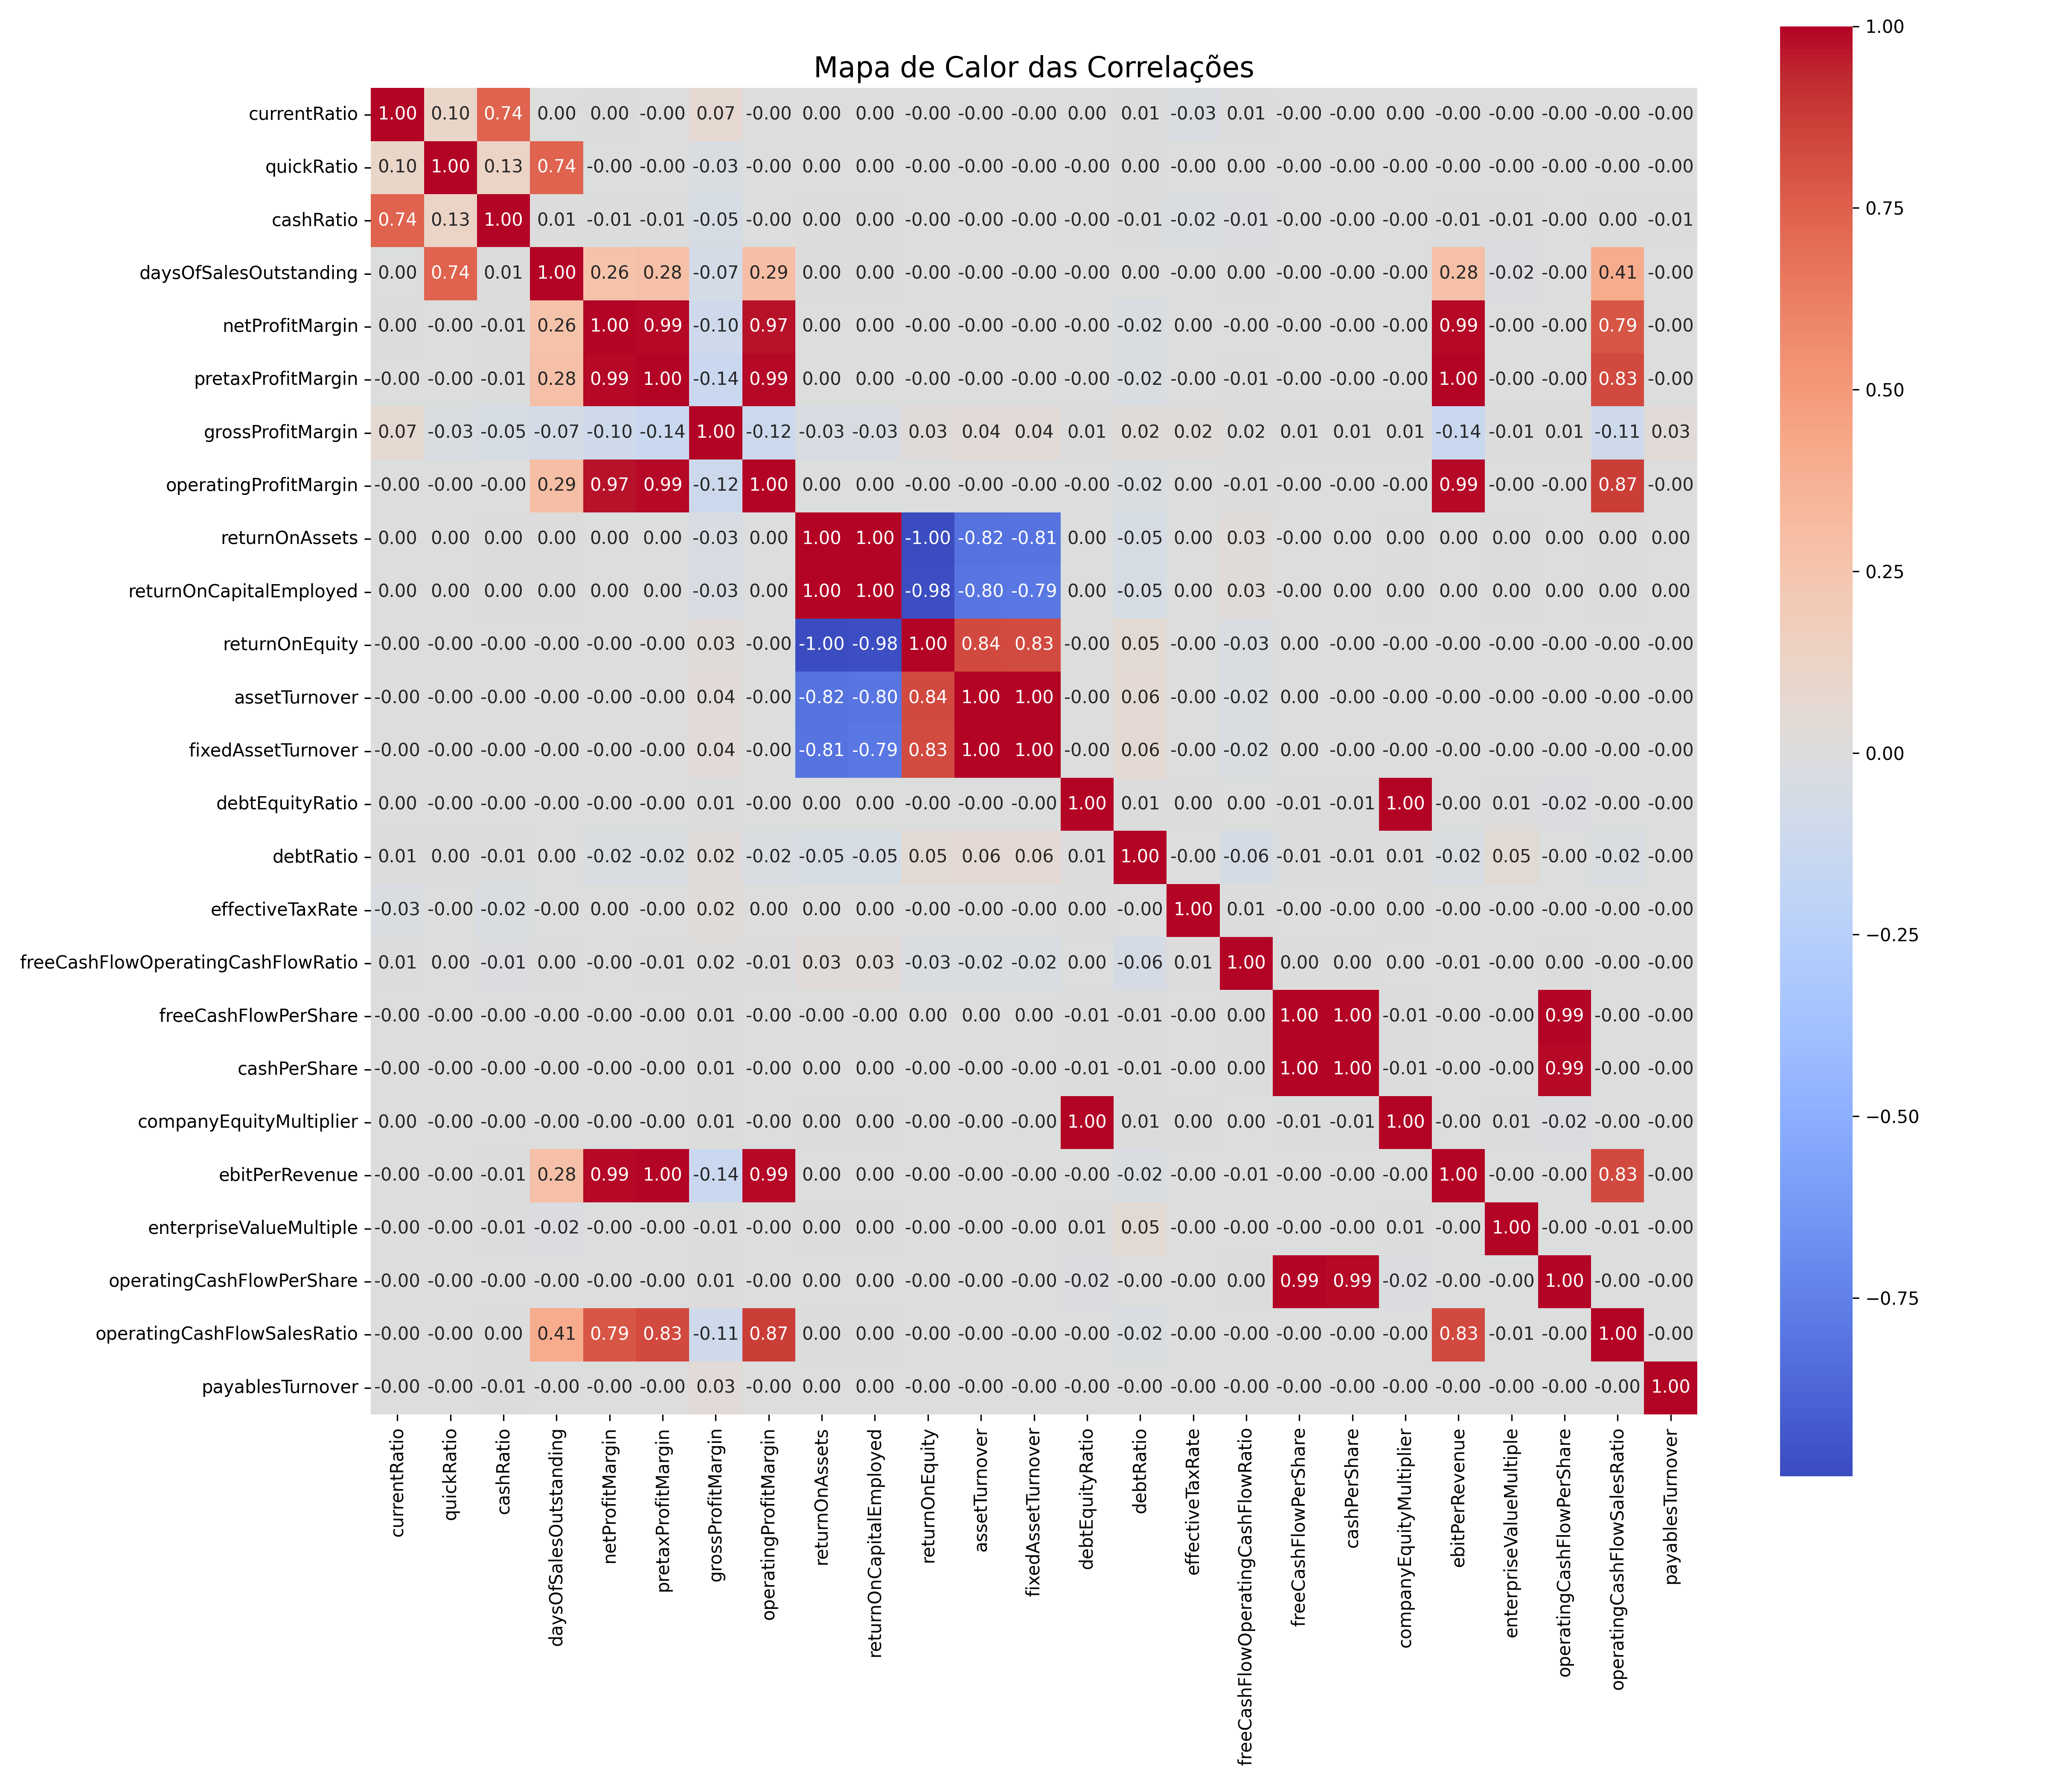
\includegraphics[width=0.85\textwidth]{figs/matriz_correlacao_inadimplencia.png}
    \caption{Matriz de correlação das variáveis do dataset \textit{Default of Credit Card Clients}.}
    \label{fig:matriz_correlacao_inadimplencia}
\end{figure}

A partir da matriz de correlação apresentada na Figura~\ref{fig:matriz_correlacao_inadimplencia}, é possível observar que as variáveis \texttt{BILL\_AMT1}, \texttt{BILL\_AMT2}, \texttt{BILL\_AMT3}, \texttt{BILL\_AMT4}, \texttt{BILL\_AMT5} e \texttt{BILL\_AMT6} possuem forte correlação entre si, caracterizando-se como colineares. Além disso, percebe-se que a variável \texttt{PAY\_5} apresenta forte correlação com \texttt{PAY\_4} e \texttt{PAY\_6}.

\subsection{Corporate Credit Rating}

O \textit{Corporate Credit Rating Dataset}, disponível no Kaggle \footnote{\url{https://www.kaggle.com/datasets/agewerc/corporate-credit-rating}}, contém 2029 registros e 31 variáveis, com dados financeiros de grandes empresas americanas listadas na NYSE e na Nasdaq entre 2010 e 2016. Destas, 30 são variáveis preditoras e uma é a variável alvo, correspondente à classificação de crédito atribuída às empresas. O conjunto inclui indicadores de liquidez, lucratividade, endividamento, fluxo de caixa e dados cadastrais, sendo utilizado para prever ratings de crédito — classificações emitidas por agências que indicam o risco de inadimplência das companhias.

As variáveis preditoras podem ser agrupadas da seguinte forma:

\begin{sloppypar}
\begin{itemize}
    \item \textbf{Índices de Liquidez:} \texttt{currentRatio}, \texttt{quickRatio}, \texttt{cashRatio}, \texttt{daysOfSalesOutstanding};
    \item \textbf{Indicadores de Lucratividade:} \texttt{grossProfitMargin}, \texttt{operatingProfitMargin}, \texttt{pretaxProfitMargin}, \texttt{netProfitMargin}, \texttt{effectiveTaxRate}, \texttt{returnOnAssets}, \texttt{returnOnEquity}, \texttt{returnOnCapitalEmployed};
    \item \textbf{Índices de Endividamento:} \texttt{debtRatio}, \texttt{debtEquityRatio};
    \item \textbf{Indicador de Desempenho Operacional:} \texttt{assetTurnover};
    \item \textbf{Indicadores de Fluxo de Caixa:} \texttt{operatingCashFlowPerShare}, \texttt{freeCashFlowPerShare}, \texttt{cashPerShare}, \texttt{operatingCashFlowSalesRatio}, \texttt{freeCashFlowOperatingCashFlowRatio}
\end{itemize}
A variável alvo, \texttt{Rating}, representa a classificação de crédito das empresas. Observa-se que esta variável está desbalanceada, com concentração significativa em poucas classes, especialmente nas categorias \textbf{BBB}, \textbf{BB} e \textbf{A}, que juntas correspondem a mais de 75\% dos registros. A Tabela~\ref{tab:dist_rating} apresenta a distribuição detalhada da variável alvo.
\end{sloppypar}

\begin{table}[H]
\centering
\caption{Distribuição da variável alvo (\texttt{Rating}) no dataset \textit{Corporate Credit Rating Dataset}}
\label{tab:dist_rating}
\begin{tabular}{lcc}
\hline
\textbf{Rating} & \textbf{Quantidade} & \textbf{Frequência (\%)} \\
\hline
BBB   & 671 & 33.07 \\
BB    & 490 & 24.15 \\
A     & 398 & 19.62 \\
B     & 302 & 14.88 \\
AA    & 89  & 4.39  \\
CCC   & 64  & 3.15  \\
AAA   & 7   & 0.34  \\
CC    & 5   & 0.25  \\
C     & 2   & 0.10  \\
D     & 1   & 0.05  \\
\hline
\textbf{Total} & 2029 & 100.00 \\
\hline
\end{tabular}
\end{table}

A seguir na Figura~\ref{fig:matriz_correlacao_corporate_credit_rating}, apresenta-se a matriz de correlação entre as variáveis do dataset:

\begin{figure}[H]
    \centering
    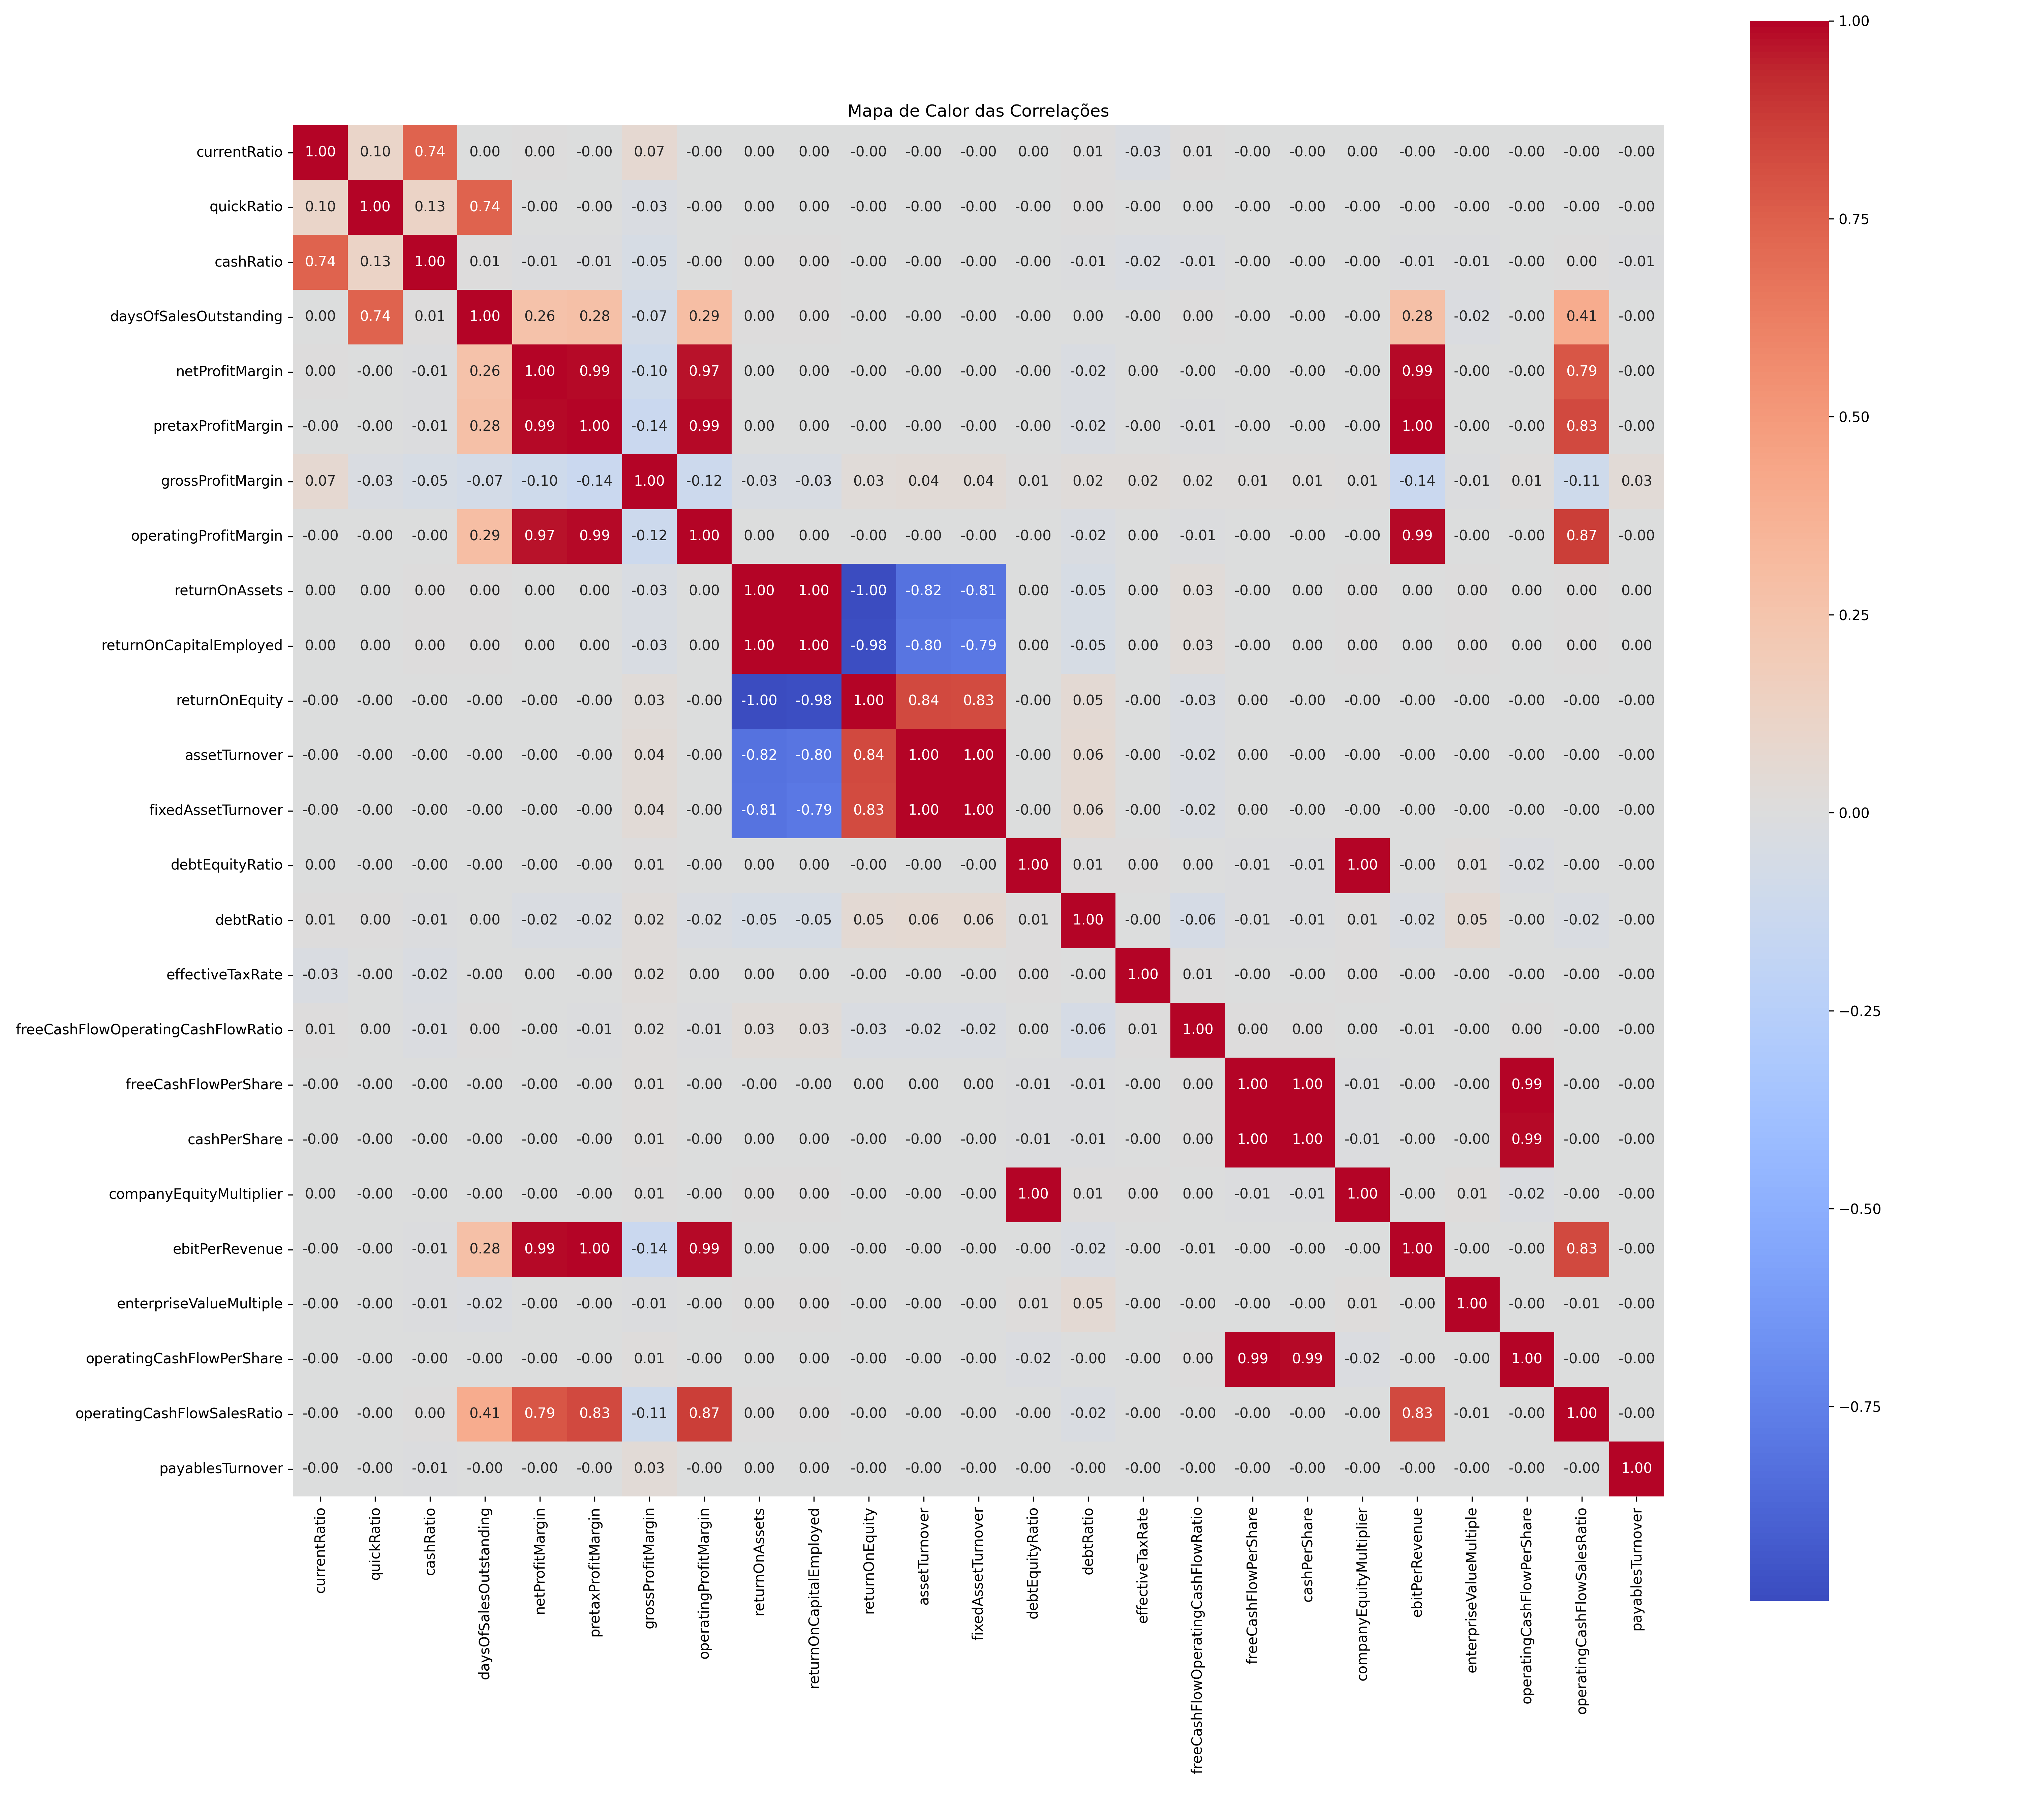
\includegraphics[width=0.85\textwidth]{figs/Correlacoes_Corporate_Credit_Rating.png}
    \caption{Matriz de correlação das variáveis do dataset \textit{Corporate Credit Rating Dataset}.}
    \label{fig:matriz_correlacao_corporate_credit_rating}
\end{figure}


\begin{sloppypar}
A partir da matriz de correlação apresentada na Figura~\ref{fig:matriz_correlacao_corporate_credit_rating}, observa-se colinearidade entre boa parte das variáveis. Destacam-se as variáveis \texttt{netProfitMargin}, \texttt{pretaxProfitMargin}, \texttt{grossProfitMargin}, \texttt{operatingProfitMargin}, \texttt{returnOnAssets}, \texttt{returnOnCapitalEmployed}, \texttt{returnOnEquity}, \texttt{assetTurnover}, \texttt{fixedAssetTurnover}, \texttt{debtEquityRatio}, \texttt{freeCashFlowPerShare}, \texttt{cashPerShare}, \texttt{companyEquityMultiplier}, \texttt{ebitPerRevenue}, \texttt{operatingCashFlowPerShare} e \texttt{operatingCashFlowSalesRatio}, que possuem correlação maior ou igual a 0,8 com uma ou mais variáveis preditoras.
\end{sloppypar}


\subsection{Conjunto de dados sintéticos}
Assim como em \citeonline{Salih2025AdditiveEffects}, o conjunto de dados sintético foi gerado utilizando o método \texttt{make\_classification} da biblioteca Scikit-learn, com os mesmos parâmetros utilizados no trabalho citado. Foram geradas 100 mil amostras com 16 variáveis preditoras (todas numéricas), nomeadas de \texttt{f1} a \texttt{f16}, das quais nove são informativas, cinco redundantes e duas representam ruído. Para introduzir diferentes níveis de colinearidade, foram adicionadas quatro novas variáveis (\texttt{f17}, \texttt{f18}, \texttt{f19} e \texttt{f20}) como combinações lineares de \texttt{f1}, \texttt{f2}, \texttt{f3} e \texttt{f4}, respectivamente.A variável alvo é balanceada e apresenta apenas duas classes, 0 ou 1.

A Figura~\ref{fig:matriz_correlacao_dados_sinteticos} apresenta matriz de correlação dos dados:

\begin{figure}[H]
    \centering
    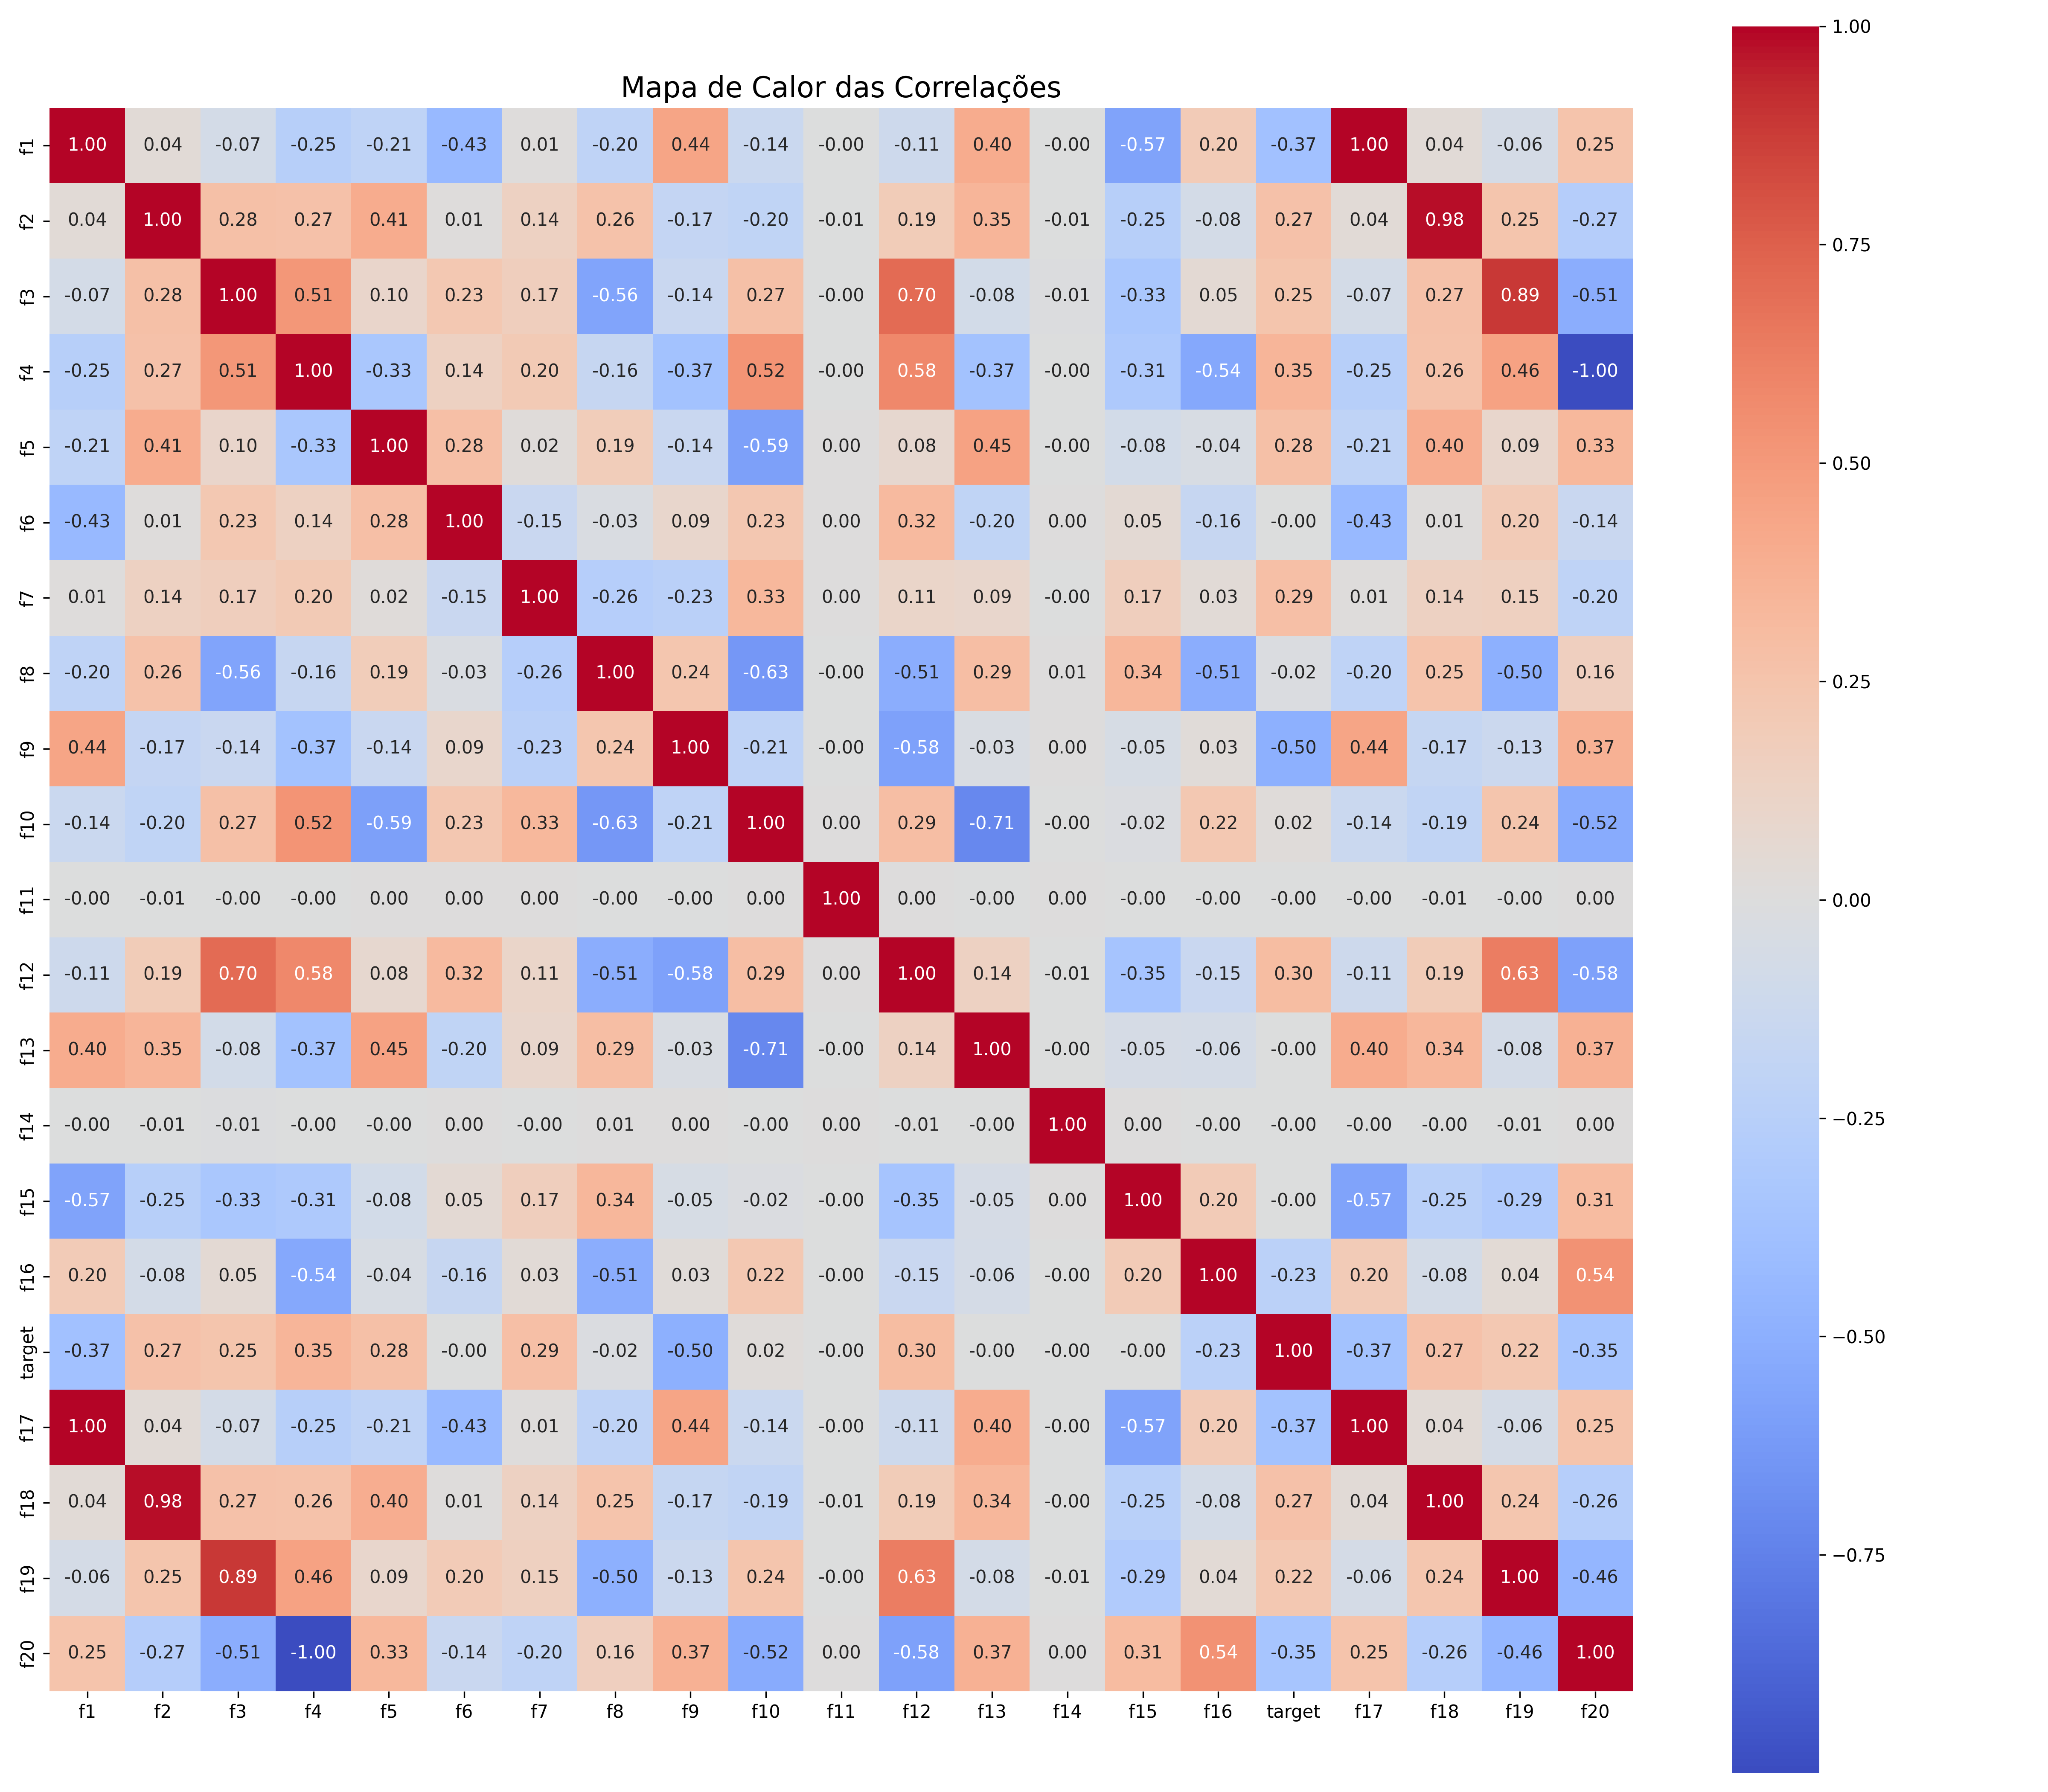
\includegraphics[width=0.85\textwidth]{figs/matriz_correlacao_dados_sinteticos.png}
    \caption{Matriz de correlação das variáveis do conjunto de dados sintéticos.}
    \label{fig:matriz_correlacao_dados_sinteticos}
\end{figure}


\section{Configuração do experimento}\label{sec:cofiguracao_experimentos}
Os conjuntos de dados serão divididos em dados de treino (70\%) e teste (30\%). Para cada conjunto, serão treinados e avaliados quatro algoritmos de classificação: SVM, Random Forest, LightGBM e XGBoost. Esses algoritmos foram escolhidos por serem amplamente utilizados, não serem naturalmente explicáveis e atenderem às limitações de recursos computacionais disponíveis para este trabalho. A implementação será realizada com a biblioteca Scikit-learn \cite{scikit-learn}, utilizando inicialmente os parâmetros padrão de cada modelo.

O desempenho preditivo dos algoritmos será avaliado com as métricas F1-score e ROC AUC, também disponíveis na biblioteca Scikit-learn \cite{scikit-learn}. Essas métricas permitem uma avaliação equilibrada do desempenho geral do modelo, sem penalizar excessivamente falsos negativos ou falsos positivos. Após o treinamento e avaliação, serão aplicadas as técnicas SHAP e LIME, por meio das bibliotecas shap e lime, respectivamente, para gerar explicações sobre as decisões dos modelos. A estabilidade das explicações será avaliada por meio da métrica NMR (\textit{Normalized Movement Rate}).

Posteriormente, o experimento será repetido utilizando dados transformados por PCA e dados com variáveis redundantes removidas, permitindo comparar o impacto da colinearidade na estabilidade das explicações geradas.





	
	% PARTE - Define a divisão do documento em partes (Não é obrigatório)
	%\part{Preparação da pesquisa}
	%% ---
\chapter{Uso de referências bibliográficas}
% ---

A formatação das referências bibliográficas conforme as regras da ABNT são um
dos principais objetivos do \abnTeX. Consulte os manuais
\citeonline{abntex2cite} e \citeonline{abntex2cite-alf} para obter informações
sobre como utilizar as referências bibliográficas.

%-
\subsection{Acentuação de referências bibliográficas}
%-

Normalmente não há problemas em usar caracteres acentuados em arquivos
bibliográficos (\texttt{*.bib}). Na~\autoref{tabela-acentos} você encontra alguns exemplos das conversões mais importantes. Preste atenção especial para `ç' e `í'
que devem estar envoltos em chaves. A regra geral é sempre usar a acentuação
neste modo quando houver conversão para letras maiúsculas.

\begin{table}[htbp]
\caption{Tabela de conversão de acentuação.}
\label{tabela-acentos}

\begin{center}
\begin{tabular}{ll}\hline\hline
acento & \textsf{bibtex}\\
à á ã & \verb+\`a+ \verb+\'a+ \verb+\~a+\\
í & \verb+{\'\i}+\\
ç & \verb+{\c c}+\\
\hline\hline
\end{tabular}
\end{center}
\end{table}


% ---
\section{Deu pau em algo?}
% ---

Consulte a FAQ com perguntas frequentes e comuns no portal do \abnTeX:
\url{https://code.google.com/p/abntex2/wiki/FAQ}.

Inscreva-se no grupo de usuários \LaTeX:
\url{http://groups.google.com/group/latex-br}, tire suas dúvidas e ajude a galera se tiver tudo certo.



	%\chapter{Estado da Arte}\label{cap:estArte}

\lipsum[34]

\section*{Trabalhos Relacionados a Isto}\label{sec:primTrab}
\addcontentsline{toc}{section}{Trabalhos Relacionados a Isto}

\lipsum[34-36]
	%\chapter{Materiais e Métodos}\label{cap:ferramentas}

\lipsum[43-45]

\section{Considerações Finais}

\lipsum[23]

	
	% PARTE
	%\part{Proposta}
	%\chapter{Sistema Proposto}\label{cap:proposta}

Esse trabalho propõe um sistema de... 


\section{Primeira Parte do Sistema Proposto}

\lipsum[67]

\section{Considerações Finais}

\lipsum[68]

	
	% PARTE
	%\part{Parte Final}
	%\chapter{Resultados e Discussão}\label{cap:resultados}

\lipsum[73]

\section{Base de Dados}

\lipsum[72]

\section{Considerações Finais}

\lipsum[74]
	%\chapter*{Conclusões e Trabalhos Futuros}\label{cap:conclusao}
\addcontentsline{toc}{chapter}{Conclusão e Trabalhos Futuros}

\lipsum[81]

\section*{Conclusões}

\lipsum[82-84]

\section*{Trabalhos Futuros}

\lipsum[85] 
	
	% ----------------------------------------------------------
	% ELEMENTOS PÓS-TEXTUAIS (Referências, Glossário, Apêndices)
	% ----------------------------------------------------------
	%\postextual
	
	% Referências bibliográficas
	\bibliography{bibliografia}
	
	% Glossário (Consulte o manual)
	%\glossary
	
	% Apêndices
	%% ----------------------------------------------------------
% Apêndices
% ----------------------------------------------------------

% ---
% Inicia os apêndices
% ---
\begin{apendicesenv}

% Imprime uma página indicando o início dos apêndices
\partapendices

% ----------------------------------------------------------
\chapter{Primeiro Apêncice}
% ----------------------------------------------------------

\lipsum[50] % Texto qualquer. REMOVER!!

% ----------------------------------------------------------
\chapter{Segundo apêndice com título tão grande quanto se queira porque ele já faz a quebra de linha da coisa toda}
% ----------------------------------------------------------
\lipsum[51-53] % Texto qualquer. REMOVER!!

\end{apendicesenv}
% ---
	
	% Anexos
	%% ----------------------------------------------------------
% Apêndices
% ----------------------------------------------------------

% ---
% Inicia os anexos
% ---
\begin{anexosenv}

% Imprime uma página indicando o início dos anexos
\partanexos

% ---
\chapter{Nome do Primeiro Anexo}
% ---
\lipsum[30] % Texto qualquer. REMOVER!!

% ---
\chapter{Nome de Outro Anexo}
% ---

\lipsum[32] % Texto qualquer. REMOVER!!

\end{anexosenv}
	
	% Índice remissivo (Consultar manual)
	%\phantompart
	%\printindex
	
\end{document}